% (find-LATEX "2020-2-C3-P2.tex")
% (defun c () (interactive) (find-LATEXsh "lualatex -record 2020-2-C3-P2.tex" :end))
% (defun C () (interactive) (find-LATEXsh "lualatex 2020-2-C3-P2.tex" "Success!!!"))
% (defun D () (interactive) (find-pdf-page      "~/LATEX/2020-2-C3-P2.pdf"))
% (defun d () (interactive) (find-pdftools-page "~/LATEX/2020-2-C3-P2.pdf"))
% (defun e () (interactive) (find-LATEX "2020-2-C3-P2.tex"))
% (defun o () (interactive) (find-LATEX "2020-2-C3-P2.tex"))
% (defun u () (interactive) (find-latex-upload-links "2020-2-C3-P2"))
% (defun v () (interactive) (find-2a '(e) '(d)))
% (defun d0 () (interactive) (find-ebuffer "2020-2-C3-P2.pdf"))
% (defun cv () (interactive) (C) (ee-kill-this-buffer) (v) (g))
%          (code-eec-LATEX "2020-2-C3-P2")
% (find-pdf-page   "~/LATEX/2020-2-C3-P2.pdf")
% (find-sh0 "cp -v  ~/LATEX/2020-2-C3-P2.pdf /tmp/")
% (find-sh0 "cp -v  ~/LATEX/2020-2-C3-P2.pdf /tmp/pen/")
%     (find-xournalpp "/tmp/2020-2-C3-P2.pdf")
%   file:///home/edrx/LATEX/2020-2-C3-P2.pdf
%               file:///tmp/2020-2-C3-P2.pdf
%           file:///tmp/pen/2020-2-C3-P2.pdf
% http://angg.twu.net/LATEX/2020-2-C3-P2.pdf
% (find-LATEX "2019.mk")
% (find-CN-aula-links "2020-2-C3-P2" "3" "c3m202p2" "c2p2")
%
% Video:
% (find-ssr-links "c3m202p2" "2020-2-C3-P2")
% (code-video     "c3m202p2video" "$S/http/angg.twu.net/eev-videos/2020-2-C3-P2.mp4")
% (find-c3m202p2video "0:00")

% «.defs»		(to "defs")
% «.defs-T-and-B»	(to "defs-T-and-B")
% «.title»		(to "title")
% «.regras-e-dicas»	(to "regras-e-dicas")
% «.questao-1»		(to "questao-1")
% «.questao-1-abcd»	(to "questao-1-abcd")
% «.questao-1-e»	(to "questao-1-e")
% «.figura-1.2»		(to "figura-1.2")
% «.questao-1-fgh»	(to "questao-1-fgh")
% «.questao-1-i»	(to "questao-1-i")
% «.questao-1-dica»	(to "questao-1-dica")
% «.questao-2»		(to "questao-2")
%
% «.djvuize»		(to "djvuize")

\documentclass[oneside,12pt]{article}
\usepackage[colorlinks,citecolor=DarkRed,urlcolor=DarkRed]{hyperref} % (find-es "tex" "hyperref")
\usepackage{amsmath}
\usepackage{amsfonts}
\usepackage{amssymb}
\usepackage{pict2e}
\usepackage[x11names,svgnames]{xcolor} % (find-es "tex" "xcolor")
\usepackage{colorweb}                  % (find-es "tex" "colorweb")
%\usepackage{tikz}
%
% (find-dn6 "preamble6.lua" "preamble0")
%\usepackage{proof}   % For derivation trees ("%:" lines)
%\input diagxy        % For 2D diagrams ("%D" lines)
%\xyoption{curve}     % For the ".curve=" feature in 2D diagrams
%
\usepackage{edrx15}               % (find-LATEX "edrx15.sty")
\input edrxaccents.tex            % (find-LATEX "edrxaccents.tex")
\input edrxchars.tex              % (find-LATEX "edrxchars.tex")
\input edrxheadfoot.tex           % (find-LATEX "edrxheadfoot.tex")
\input edrxgac2.tex               % (find-LATEX "edrxgac2.tex")
%
%\usepackage[backend=biber,
%   style=alphabetic]{biblatex}            % (find-es "tex" "biber")
%\addbibresource{catsem-slides.bib}        % (find-LATEX "catsem-slides.bib")
%
% (find-es "tex" "geometry")
\usepackage[a6paper, landscape,
            top=1.5cm, bottom=.25cm, left=1cm, right=1cm, includefoot
           ]{geometry}
%
\begin{document}

%\catcode`\^^J=10
%\directlua{dofile "dednat6load.lua"}  % (find-LATEX "dednat6load.lua")

% %L dofile "edrxtikz.lua"  -- (find-LATEX "edrxtikz.lua")
% %L dofile "edrxpict.lua"  -- (find-LATEX "edrxpict.lua")
% \pu

% «defs»  (to ".defs")
% (find-LATEX "edrx15.sty" "colors-2019")
\long\def\ColorRed   #1{{\color{Red1}#1}}
\long\def\ColorViolet#1{{\color{MagentaVioletLight}#1}}
\long\def\ColorViolet#1{{\color{Violet!50!black}#1}}
\long\def\ColorGreen #1{{\color{SpringDarkHard}#1}}
\long\def\ColorGreen #1{{\color{SpringGreenDark}#1}}
\long\def\ColorGreen #1{{\color{SpringGreen4}#1}}
\long\def\ColorGray  #1{{\color{GrayLight}#1}}
\long\def\ColorGray  #1{{\color{black!30!white}#1}}
\long\def\ColorBrown #1{{\color{Brown}#1}}
\long\def\ColorBrown #1{{\color{brown}#1}}
\long\def\ColorOrange#1{{\color{orange}#1}}

\long\def\ColorShort #1{{\color{SpringGreen4}#1}}
\long\def\ColorLong  #1{{\color{Red1}#1}}

\def\frown{\ensuremath{{=}{(}}}
\def\True {\mathbf{V}}
\def\False{\mathbf{F}}
\def\D    {\displaystyle}

\def\drafturl{http://angg.twu.net/LATEX/2020-2-C3.pdf}
\def\drafturl{http://angg.twu.net/2020.2-C3.html}
\def\draftfooter{\tiny \href{\drafturl}{\jobname{}} \ColorBrown{\shorttoday{} \hours}}

\def\gradF{\Vec{∇F}}

% «defs-T-and-B»  (to ".defs-T-and-B")
% (c3m202p1p 6 "questao-2")
% (c3m202p1    "questao-2")
\def\T(Total: #1 pts){{\bf(Total: #1)}}
\def\T(Total: #1 pts){{\bf(Total: #1 pts)}}
\def\T(Total: #1 pts){\ColorRed{\bf(Total: #1 pts)}}
\def\B       (#1 pts){\ColorOrange{\bf(#1 pts)}}





%  _____ _ _   _                               
% |_   _(_) |_| | ___   _ __   __ _  __ _  ___ 
%   | | | | __| |/ _ \ | '_ \ / _` |/ _` |/ _ \
%   | | | | |_| |  __/ | |_) | (_| | (_| |  __/
%   |_| |_|\__|_|\___| | .__/ \__,_|\__, |\___|
%                      |_|          |___/      
%
% «title»  (to ".title")
% (c3m202p2p 1 "title")
% (c3m202p2    "title")

\thispagestyle{empty}

\begin{center}

\vspace*{1.2cm}

{\bf \Large Cálculo 3 - 2020.2}

\bsk

P2 (segunda prova)

\bsk

Eduardo Ochs - RCN/PURO/UFF

\url{http://angg.twu.net/2020.2-C3.html}

\end{center}

\newpage

% «regras-e-dicas»  (to ".regras-e-dicas")
% (c3m202p2p 2 "regras-e-dicas")
% (c3m202p2    "regras-e-dicas")

{\bf Regras e dicas}

As regras e dicas são as mesmas dos mini-testes e da P1:

\ssk

\url{http://angg.twu.net/LATEX/2020-2-C3-MT1.pdf}

\url{http://angg.twu.net/LATEX/2020-2-C3-MT2.pdf}

\url{http://angg.twu.net/LATEX/2020-2-C3-P1.pdf}

\ssk

exceto que a prova foi disponibilizada às 16:45 do dia

1º/maio/2021 e deve ser entregue até as 14:00 do dia

3/maio/2021.



\newpage

% «questao-1»  (to ".questao-1")
% (c3m202p2p 3 "questao-1")
% (c3m202p2     "questao-1")
% (c3m202planotangp 31 "grad-intro")
% (c3m202planotang     "grad-intro")

{\bf Questão 1.}

\T(Total: 9.0 pts)

% a 0.4
% b 0.3
% c 0.3
% d 0.5  -> 1.5
% 
% e 1.0
%
% f 1.5
% g 1.5
% h 1.5
%
% i 2.0

Esta questão é baseada neste material manuscrito sobre

vetor gradiente, que discutimos na aula de 30 de maio:

\ssk

{\footnotesize

% http://angg.twu.net/LATEX/2020-2-C3-plano-tang.pdf#page=31
\url{http://angg.twu.net/LATEX/2020-2-C3-plano-tang.pdf\#page=31}

}

\ssk

Esta aqui é a Figura 1.1:
%
$$
% (find-latexscan-links "C3" "20210430_grad_superficie_orig")
% (find-xpdf-page "~/LATEX/2020-2-C3/20210430_grad_superficie_orig.pdf")
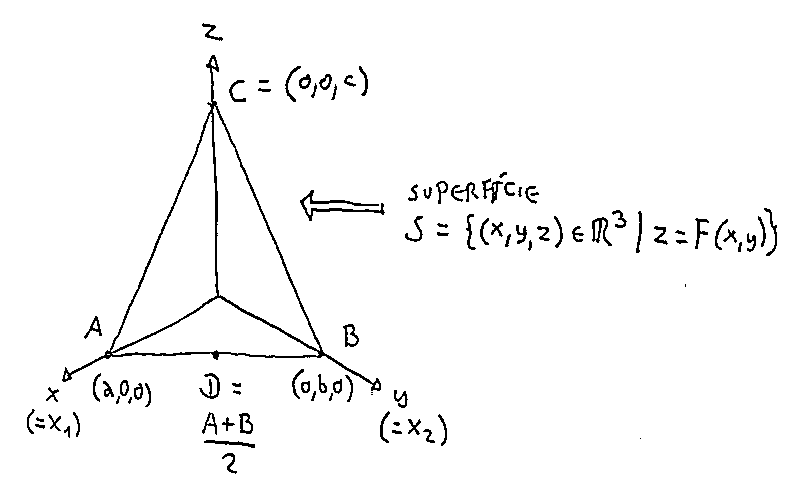
\includegraphics[height=4cm]{2020-2-C3/20210430_grad_superficie_orig.pdf}
$$

\newpage

% «questao-1-abcd»  (to ".questao-1-abcd")
% (c3m202p2p 4 "questao-1-abcd")
% (c3m202p2    "questao-1-abcd")

{\bf Questão 1 (cont.)}

\ssk

a) \B(0.4 pts) Encontre uma fórmula para a função $F(x,y)$.

\ssk

b) \B(0.3 pts) Calcule as derivadas parciais $F_x(x_0,y_0)$ e $F_y(x_0,y_0)$.

Você deve obter expressões que não dependem de $x_0$ ou de $y_0$.

\msk

Para cada ponto $P$ de $\R^3$ nós vamos denotar por $P_0$ a sua

projeção no plano $π_{xy}$: se $P=(x,y,z)$ então $P_0=(x,y)$.

c) \B(0.3 pts) Diga as coordenadas de $D$ e de $D_0$.

\bsk

O exercício 7 do PDF de planos tangentes é sobre como

entender a definição de matriz jacobiana do livro do

Bortolossi, na notação dele.

\ssk

d) \B(0.5 pts) Digamos que $𝐛f=F$ e $𝐛p=D_0$. Calcule $D𝐛f(𝐛p)$

($= DF(D_0)$). O resultado deve ser uma matriz $1×2$ cujas

entradas são expressões que não dependem de $x_0$ ou de $y_0$.

\newpage

% «questao-1-e»  (to ".questao-1-e")
% (c3m202p2p 5 "questao-1-e")
% (c3m202p2    "questao-1-e")

{\bf Questão 1 (cont.)}

\ssk

e) \B(1.0 pts) Leia a definição de vetor gradiente na seção 8.2 do

Bortolossi (no cap.8) e calcule $∇F(D)$. Você deve obter um

vetor em $\R^2$ cujas componentes são expressões que só dependem

de $a$, $b$ e $c$.

\msk

Obs: note que o Bortolossi escreve
%
$$f: D⊂\R^n → \R$$

onde $D$ é o domínio da função $f$. Nós estamos sempre usando

a função
%
$$F: \R^2 → \R$$

e o domínio dela é o $\R^2$ inteiro... isso nos libera pra

usar o símbolo $D$ pra outras coisas.

\newpage

% «figura-1.2»  (to ".figura-1.2")
% (c3m202p2p 6 "figura-1.2")
% (c3m202p2     "figura-1.2")

Isto aqui é a nossa Figura 1.2:

% (find-latexscan-links "C3" "20210430_C3_P2_fig_1.2")
% (find-xpdf-page "~/LATEX/2020-2-C3/20210430_C3_P2_fig_1.2.pdf")
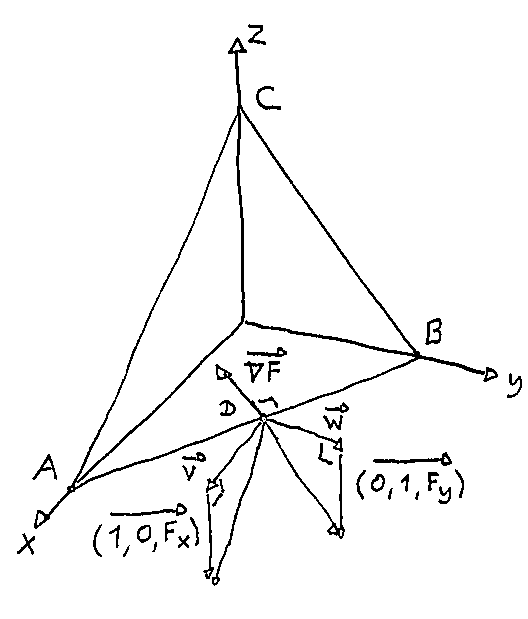
\includegraphics[height=7.0cm]{2020-2-C3/20210430_C3_P2_fig_1.2.pdf}

\newpage

...ou melhor, a figura da página anterior é {\sl uma versão} da Figura
1.2; já vou explicar porquê.

Nos slides 23 a 25 do PDF sobre planos tangentes nós vimos uma figura
que pra desenhá-la com todos os detalhes nós tivemos que desmontá-la
em várias, fazer um zoom numa parte dela e escrever certas coisas só
na versão zoomada. Na figura 1.2 vai acontecer a mesma coisa: pra
conseguir desenhar e escrever todos os detalhes nela você
provavelmente vai ter que fazer pelo menos uma figura como a do slide
anterior e uma outra só com o que está perto do ponto $D$.

Note que os dois triângulos abaixo e à direita são triângulos
retângulos --- os sinais ``$\pbsymbol{5}$'' indicam ângulo reto --- e
eles são derivadas interpretadas como triângulos, como no PDF de
planos tangentes nos slides 22 a 30. Eu acabei não escrevendo isso no
desenho, mas $\vv = \VEC{1,0,0}$ e $\ww = \VEC{0,1,0}$. O vetor
gradiente $∇F(D)$ está escrito como $\gradF$.

% (c3m202planotangp 22 "derivs-como-triangs")
% (c3m202planotang     "derivs-como-triangs")

\newpage

{\bf Questão 1 (cont.)}

Na figura 1.2 eu pus um sinal de ângulo reto no $\gradF$ pra indicar
que $\gradF ⊥ \Vec{AB}$, ou seja, que os vetores $\gradF$ e $\Vec{AB}$
são vetores ortogonais em $\R^2$ --- ou seja, que $\gradF·\Vec{AB} =
0$. Uma das propriedades mais famosas do gradiente é que ele é sempre
ortogonal às curvas de nível; nos próximos itens nós vamos tentar
entender o que isso quer dizer geometricamente, e porque isto é
verdade.

\bsk

Obs: acho que o Bortolossi nunca diz explicitamente, em português, que
o (campo) gradiente é ortogonal às curvas de nível; mas isso é uma
consequência fácil do que ele diz na página 302, e de certas
igualdades envolvendo cossenos que ele demonstra que são verdadeiras.


\newpage

% «questao-1-fgh»  (to ".questao-1-fgh")
% (c3m202p2p 9 "questao-1-fgh")
% (c3m202p2    "questao-1-fgh")

{\bf Questão 1 (cont.)}

\msk

f) \B(1.5 pts) Faça uma versão da Figura 1.2 para o caso em que
$a=b=c=4$ (vou chamar isto de ``caso particular 1'').

\msk

Mais precisamente: faça uma versão melhorada da ``Figura 1.2 para o
caso $a=b=c=4$'' que eu fiz à mão às pressas durante a última aula e
pus no slide 33 do PDF de planos tangentes. Inclua a fórmula para
calcular $F(x,y)$ no caso $a=b=c=4$, os valores das derivadas parciais
$F_x$ e $F_y$, e o que mais você achar relevante. Lembre que você {\sl
  pode} fazer uma versão zoomada da parte perto do ponto $D$ em
separado!

Use o mesmo nível de detalhe nos itens (g) e (h) abaixo.

\msk

g) \B(1.5 pts) Faça uma versão da Figura 1.2 para o caso em que
$a=4$ e $b=c=2$ (``caso particular 2'').

h) \B(1.5 pts) Faça uma versão da Figura 1.2 para o caso em que
$a=4$, $b=4$ e $c=3$ (``caso particular 3'').


\newpage

% «questao-1-i»  (to ".questao-1-i")
% (c3m202p2p 10 "questao-1-i")
% (c3m202p2     "questao-1-i")

{\bf Questão 1 (cont.)}

\ssk

Nos slides 10 em diante do PDF sobre planos tangentes vocês aprenderam
a fazer figuras que representam casos gerais.

\msk

i) \B(2.0 pts) Faça uma versão da figura que você fez no item versão
(h) mas que ``represente o caso geral'', como na figura do slide 10 de
planos tangentes, e ponha do lado dela as contas que mostram que
$\Vec{AB}·\gradF = 0$.

% (c3m202planotangp 10 "geral-e-particular")
% (c3m202planotang     "geral-e-particular")



\newpage

% «questao-1-dica»  (to ".questao-1-dica")
% (c3m202p2p 11 "questao-1-dica")
% (c3m202p2     "questao-1-dica")

{\bf Dica pra questão 1d: use tipos!}

O Bortolossi usa ``$D$'' com vários significados diferentes --- por
exemplo, como derivada e como domínio de uma função --- e nessa
questão a gente está usando tanto a notação dele quanto a minha, então
a gente tem que saber resolver as ambiguidades... um dos jeitos que eu
acho melhores pra isso é fazendo diagramas com chaves, como esse aqui,
e indicando o ``tipo'' de cada subexpressão...

% (find-latexscan-links "C3" "20210501_C3_P2_dica")
% (find-xpdf-page "~/LATEX/2020-2-C3/20210501_C3_P2_dica.pdf")
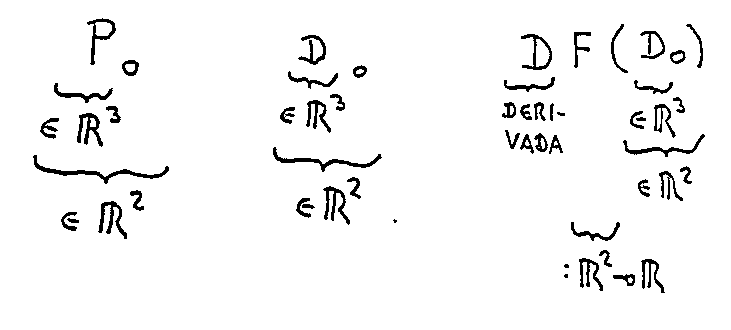
\includegraphics[height=3.5cm]{2020-2-C3/20210501_C3_P2_dica.pdf}

\newpage

A gente chegou a fazer um exercício sobre isso:

% http://angg.twu.net/LATEX/2020-2-C3-rcadeia1.pdf#page=31
\url{http://angg.twu.net/LATEX/2020-2-C3-rcadeia1.pdf\#page=31}

\msk

Vejam se a figura do slide anterior ajuda --- e lembrem de prestar
{\sl muita} atenção nas fontes. Em livros de matemática um $P$ em
itálico costuma ser algo totalmente diferente de um $𝐛P$ em boldface,
e um $P$ maiúsculo costuma ser algo totalmente diferente de um $p$
minúsculo...

\msk

Às vezes a gente tem que refazer o diagrama de tipos várias vezes até
encontrar uma interpretação pra cada subexpressão que faça sentido.
${=}($




\newpage

% «questao-2»  (to ".questao-2")
% (c3m202p2p 13 "questao-2")
% (c3m202p2     "questao-2")
% (c3m202planotangp 28 "exercicio-10")
% (c3m202planotang     "exercicio-10")

{\bf Questão 2.}

\T(Total: 3.0 pts)

\msk

a) \B(1.0 pts) Faça o exercício (10a) do PDF de planos tangentes.

b) \B(2.0 pts) Mostre como interpretar no desenho a expressão:
%
$$F(x_0,y_0) +
    \bmat{F_x(x_0,y_0) & F_y(x_0,y_0)} · \bmat{α \\ β} \, .
$$

% F(x_0+α, y_0+β) = 
% Dica: mostre como 


% (c3m202planotangp 31 "grad-intro")
% (c3m202planotang     "grad-intro")



%\printbibliography

\GenericWarning{Success:}{Success!!!}  % Used by `M-x cv'

\end{document}

%  ____  _             _         
% |  _ \(_)_   ___   _(_)_______ 
% | | | | \ \ / / | | | |_  / _ \
% | |_| | |\ V /| |_| | |/ /  __/
% |____// | \_/  \__,_|_/___\___|
%     |__/                       
%
% «djvuize»  (to ".djvuize")
% (find-LATEXgrep "grep --color -nH --null -e djvuize 2020-1*.tex")

 (eepitch-shell)
 (eepitch-kill)
 (eepitch-shell)
# (find-fline "~/2020.2-C3/")
# (find-fline "~/LATEX/2020-2-C3/")
# (find-fline "~/bin/djvuize")

cd /tmp/
for i in *.jpg; do echo f $(basename $i .jpg); done

f () { rm -fv $1.png $1.pdf; djvuize $1.pdf }
f () { rm -fv $1.png $1.pdf; djvuize WHITEBOARDOPTS="-m 1.0" $1.pdf; xpdf $1.pdf }
f () { rm -fv $1.png $1.pdf; djvuize WHITEBOARDOPTS="-m 0.5" $1.pdf; xpdf $1.pdf }
f () { rm -fv $1.png $1.pdf; djvuize WHITEBOARDOPTS="-m 0.25" $1.pdf; xpdf $1.pdf }
f () { cp -fv $1.png $1.pdf       ~/2020.2-C3/
       cp -fv        $1.pdf ~/LATEX/2020-2-C3/
       cat <<%%%
% (find-latexscan-links "C3" "$1")
%%%
}

f 20210430_C3_P2_fig_1.2
f 20210501_C3_P2_dica



%  __  __       _        
% |  \/  | __ _| | _____ 
% | |\/| |/ _` | |/ / _ \
% | |  | | (_| |   <  __/
% |_|  |_|\__,_|_|\_\___|
%                        
% <make>

 (eepitch-shell)
 (eepitch-kill)
 (eepitch-shell)
# (find-LATEXfile "2019planar-has-1.mk")
make -f 2019.mk STEM=2020-2-C3-P2 veryclean
make -f 2019.mk STEM=2020-2-C3-P2 pdf

% Local Variables:
% coding: utf-8-unix
% ee-tla: "c3m202p2"
% End:
